\documentclass{article}
\usepackage{blindtext}
\usepackage[T1]{fontenc}
\usepackage[utf8]{inputenc}
\usepackage{hyperref}
\usepackage{graphicx}
\graphicspath{ {./imgs/} }

\title{Intelligenze Artificiose}
\author{Nicolò Posta, Tommaso Romani, Nicolò Vescera}
\date{\today}

\begin{document}
    \maketitle
    
    \tableofcontents

    \section{Agenti Intelligenti}
        \subsection{Definizione}
            Un agente è qualsiasi cosa che può percepire l'ambiente circostante tramite
            sensori e agire su di esso tramite attuatori.\newline\newline
            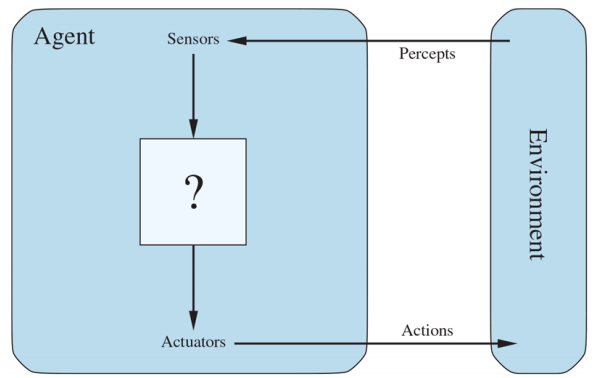
\includegraphics[scale=0.5]{agente}\\*
            Le azioni dell'agente sono influenzate dal tipo di ambiente in cui si trova.
        
        \clearpage

        \subsection{Classificazione degli Ambienti}
            Gli ambienti vengono classificati in base ai seguenti criteri:

            \begin{itemize}
                \item \textbf{Osservabilità}
                \begin{itemize}
                    \item \textbf{Fully Observable}: i sensori dell'agente gli danno accesso allo stato completo dell'ambiente in qualisasi momento.
                    \item \textbf{Partially Observable}: l'agente ha una conoscenza parziale dell'ambiente che lo circonda (può essere causato dalla limitatezza dei sensori o dalla natura stessa dell'ambiente)
                \end{itemize}
                \item \textbf{Single Agent vs Mutli Agent}: possibilità di avere un singolo agente o molteplici che possono essere \textbf{Competitivi} o \textbf{Cooperativi}
                \item \textbf{Determinabilità}:
                \begin{itemize}
                    \item \textbf{Deterministico}: lo stato successivo dell'ambiente è determinato completamente dallo stato attuale e dalle azioni effettuate dall'agente
                    \item \textbf{NON Deterministico}: tutto ciò che non è deterministo è dunque NON Deterministico (\emph{best effort !)}
                \end{itemize}
                \item \textbf{Episodico vs Sequenziale}:
                \begin{itemize}
                    \item \textbf{Episodico}: gli stati futuri non dipendono dalle azioni svolte in precedenza dall'agente (come il controllore di difetti in una linea di assemblaggio)
                    \item \textbf{Sequenziale}: il contrario di Episodico (\emph{best effort !})
                \end{itemize}
                \item \textbf{Dinamicità}:
                \begin{itemize}
                    \item \textbf{Statico}: l'ambiente cambia solamente quando l'agente effettua delle azioni
                    \item \textbf{Dinamico}: l'ambiente può cambiare mentre l'agente sta pensando
                \end{itemize}
                \item \textbf{Discreto vs Continuo}: dipende dalla maniera in cui il tempo e lo stato dell'ambiente sono gestiti dall'agente, per esempio: una partita di scacchi è discreta mentre un gioco di strategia no.
                \item \textbf{Conoscibilità}:  la conoscenza dell'agente rispetto alle leggi dell'ambiente in cui si trova.
                \textit{E.g.}: In un ambiente conosciuto data una serie di azioni si conosce il risultato.       
            \end{itemize}
    
    \section{Algoritmi di Ricerca}
\end{document}

